Los Sistemas de Almacenamiento por Baterías  ( BESS por sus siglas en inglés ) mediante el uso de  energías renovables y no convencionales son de suma importancia  para la mitigación de problemas en el suministro de energía eléctrica; a partir de las necesidades requeridas se debe realizar un diagnóstico tecnológico que permita clasificar y seleccionar  diferentes tipos de baterías adecuadas. Alrededor del mundo, se han desarrollado diferentes proyectos que se basan en los Sistemas de Almacenamiento por Baterias, entre los cuales cabe destacar:

Japón incrementó el porcentaje de nuevas energías como solar, eólica y biomasa a un 3\%; en Rokkasho se instaló un parque eólico de 51 MW de potencia nominal y un parque de baterías de Sulfuro de Sodio (NAS) con capacidad de  34 MW para mitigar las fluctuaciones generadas por energías renovables \cite{parques_eolicos}. En la Figura 2, existe una relación de los ciclos  carga/descarga de la batería evidenciando que esta compensa las fluctuaciones de la potencia eólica suministrada en un ciclo de descarga y vuelve a un estado de carga cuando la energía eólica puede mantener un nivel óptimo de potencia.
\begin{figure}[h!] %%BATERIASSECCIONES
    \begin{center}
    \centering
    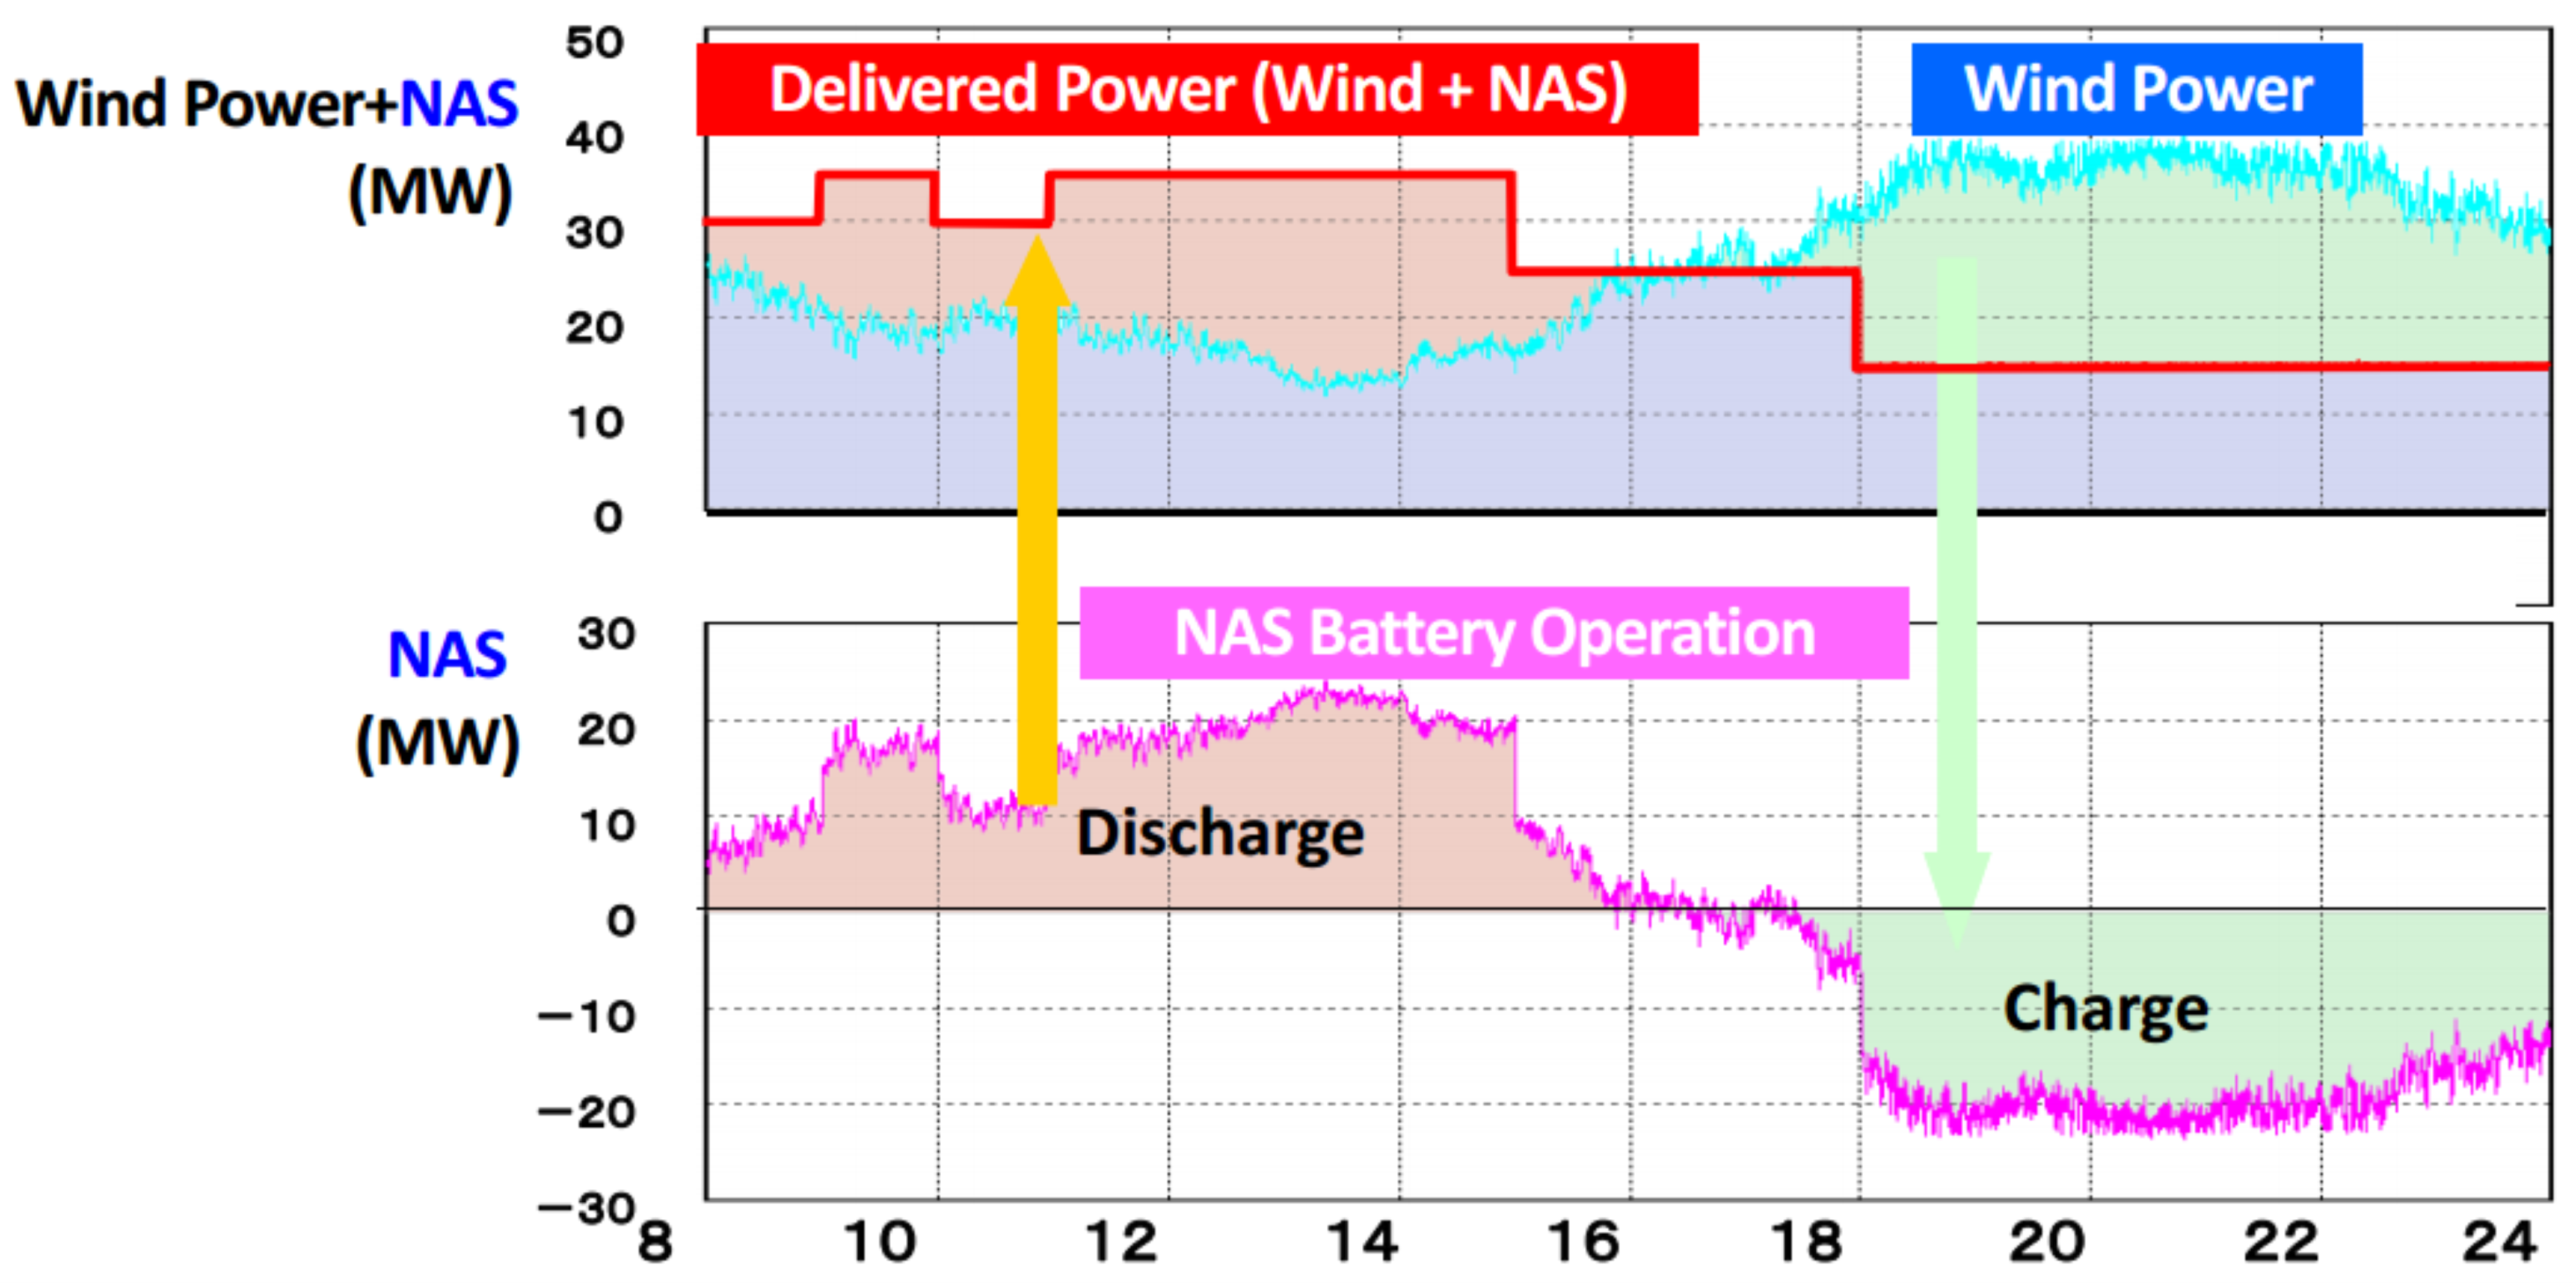
\includegraphics[scale=0.3]{Imágenes/Estado del arte/nas+wind.png}
	\caption{ Curva de generación de energía eléctrica parque eólico Rokkasho \cite{bess_zarate}}
    \end{center}
\end{figure}
\newpage
M5BAT es un sistema BESS híbrido para brindar reserva de contención de frecuencia (FCR) con potencia total de 5 MW en Alemania. El sistema está compuesto por bancos de baterías de plomo-ácido y ión-litio con una capacidad total de 5,8 MWh. \cite{BESS_GERMANY}. En la Figura 3, se realiza una comparación de potencia FCR y energía acumulada en un día así como el promedio de 12 horas en el año. El objetivo es obtener numerosas acciones de gestión energética para mejorar la comparabilidad entre el promedio de potencia y el rendimiento de energía; los resultados de laboratorio entregan una mayor potencia en promedio y un mayor rendimiento en el perfil de 12 horas debido al cambio del estado de carga de la batería durante todo el día.
\begin{figure}[h!]
    \begin{center}
    \centering
    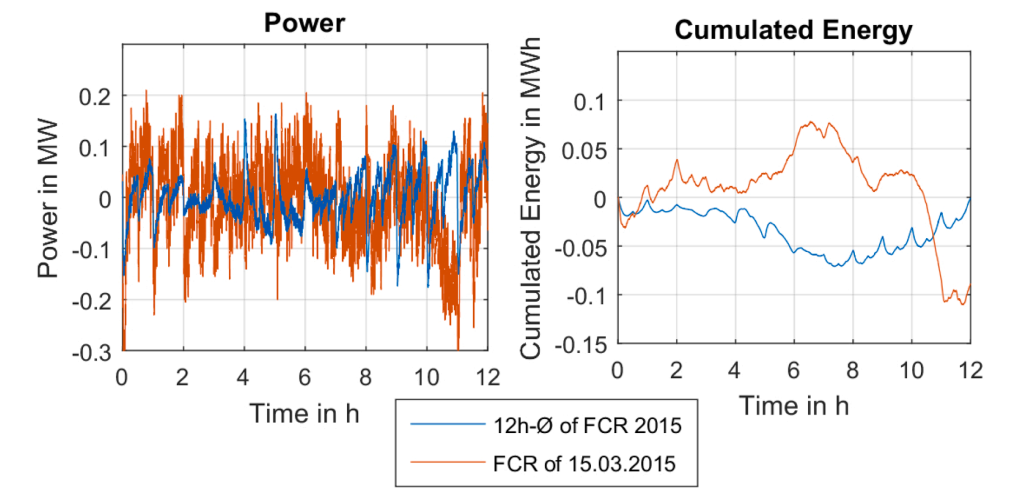
\includegraphics[scale=0.62]{Imágenes/Estado del arte/FCR ACIDO.png}
	\caption{ Comparación de potencia FCR en el año 2015 \cite{BESS_GERMANY}}
    \end{center}
\end{figure}
\newline
Los edificios consumen el 29\% de la energía en Japón; por lo tanto, para dar un aprovechamiento de la energía solar se implementó un esquema de control de potencia eficiente y un sistema independiente híbrido renovable que proporcione una salida con baja distorsión armónica. El sistema es instalado en el techo de los edificios de la ciudad de Kasuga, consiste de tres módulos de paneles solares con una potencia total de 480 W, una turbina de viento de 400 W y una batería de plomo ácido con una capacidad de 30 Ah \cite{BESS_KASUGA_JAPON}.

En la Figura 4, se visualiza la potencia promedio de salida en las fuentes de energía y la potencia consumida por la carga; el sistema de control extrae la máxima potencia del PV, la turbina y la batería en respuesta a los requerimientos de la carga. Por lo tanto, en el momento que exista un cambio en el entorno o dinámica del sistema, el sistema de control balancea el flujo de potencia de forma inmediata. 
\begin{figure}[h!]
    \begin{center}
    \centering
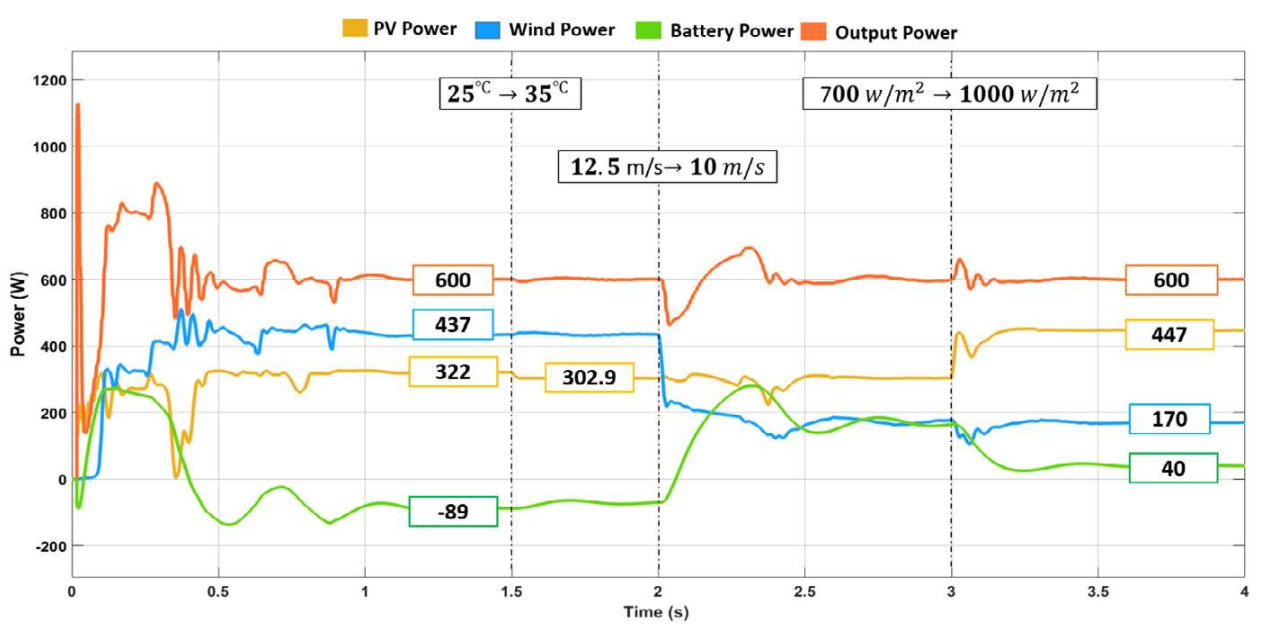
\includegraphics[scale=0.6]{Imágenes/Estado del arte/besskasuga.png}
	\caption{ Características de descarga de la batería \cite{BESS_KASUGA_JAPON}}
    \end{center}
\end{figure}

En el norte de China se implementó un proyecto para  la co-optimización de  la capacidad del sistema de almacenamiento de energía térmica y de baterías en sistema complementario de energía múltiple con plantas eólicas (300 MW), estaciones fotovoltaícas (300 MW), planta de energía termosolar (50 MW) y una batería de Ión Litio (50 MW); el sistema tiene como objetivo maximizar la utilidad anual de las energías renovables \cite{li2019capacity}.

En la Figura 5 , se visualiza la salida de cada sistema multi energía en tres días; la batería se carga durante el día cuando el suministro de energía es  proporcionado mayoritariamente por las fuentes fotovoltaícas y eólicas. De la misma forma, la descarga de la batería sucede en la noche suministrando energía eléctrica  junto con la fuente de energía solar concentrada (CSP).
\begin{figure}[h!]
    \begin{center}
    \centering
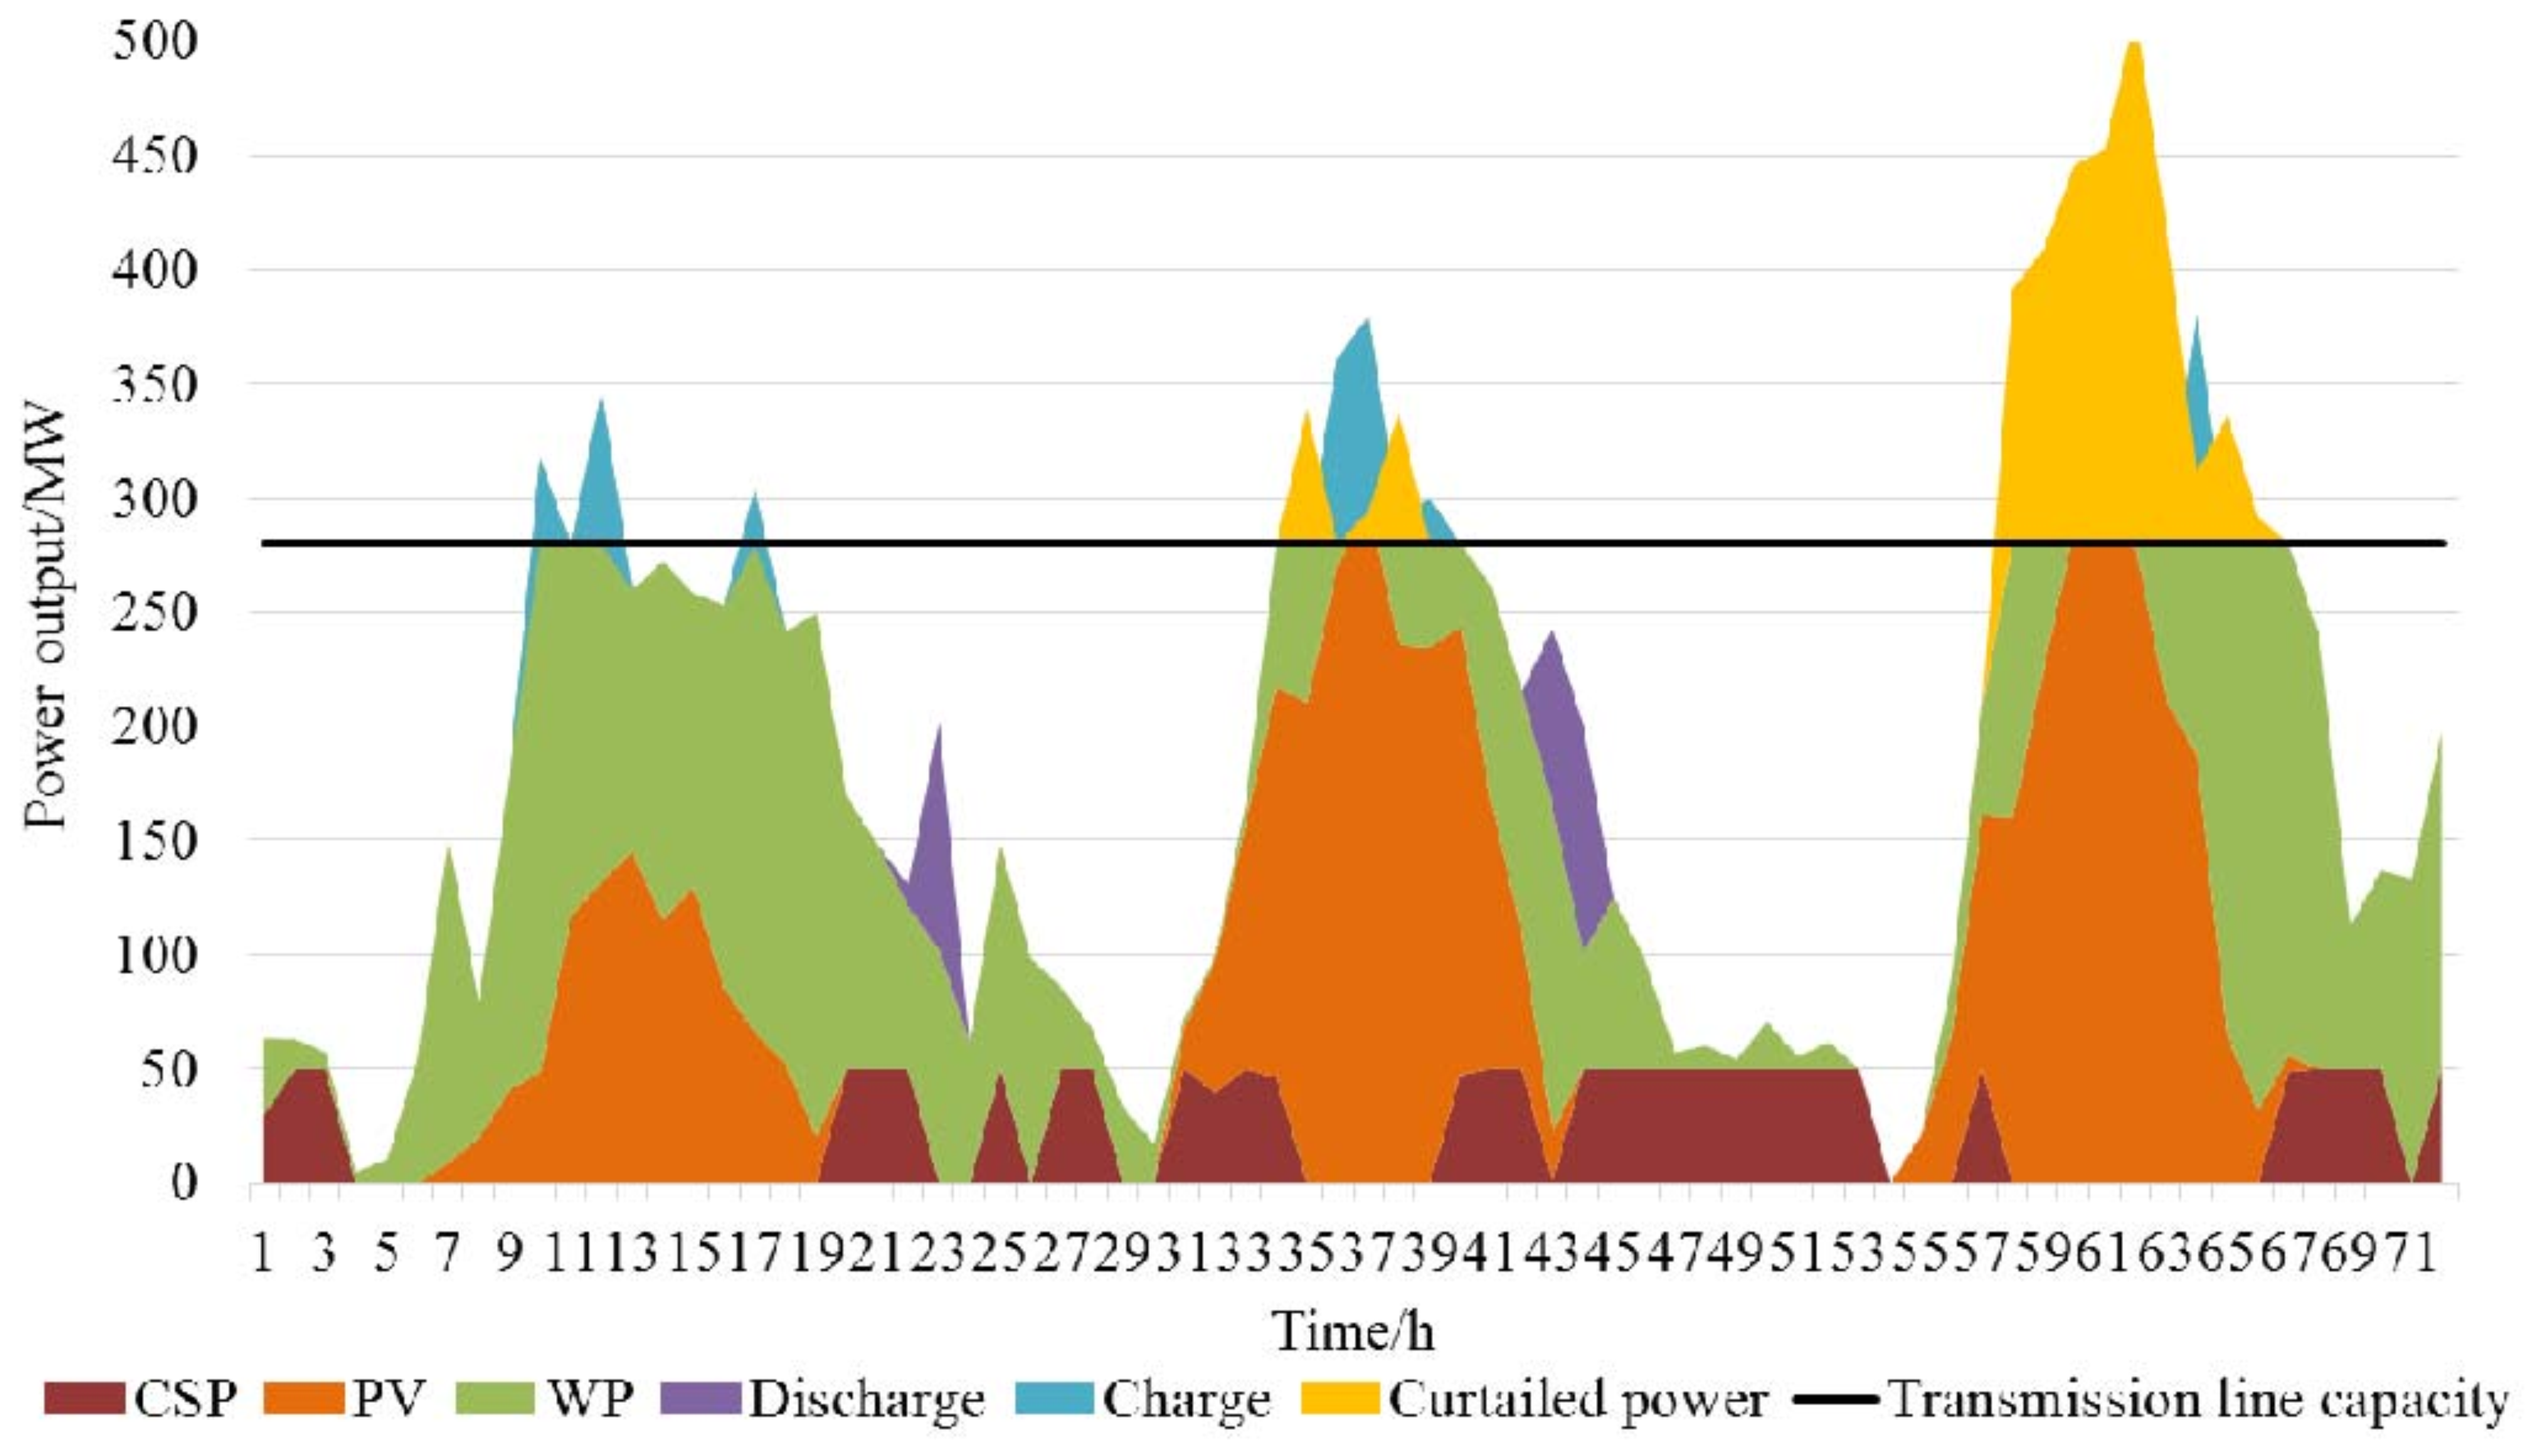
\includegraphics[scale=0.4]{Imágenes/Estado del arte/Energiatermica.png}
	\caption{Salida de potencia sistema multi energía
	\cite{li2019capacity}}
    \end{center}
\end{figure}
\newline
En Medellín-Colombia se realizó una investigación sobre la evaluación del desempeño de microrredes aisladas en áreas no interconectadas donde se analiza la integración de energía generada mediante fuentes diesel y fotovoltaicas integradas con sistemas BESS. En la figura 6 , se evidencia la media horaria de todo el año correspondiente a la energía utilizada para cargar el sistema BESS, donde el modelo prioriza la fuente fotovoltaica debido a sus bajos costos y solo se utiliza el generador diesel cuando la fuente fotovoltaica no produce la energía necesaria para caragar el sistema BESS \cite{ropero2022sizing}.
\newpage
\begin{figure}[h!]
    \begin{center}
    \centering
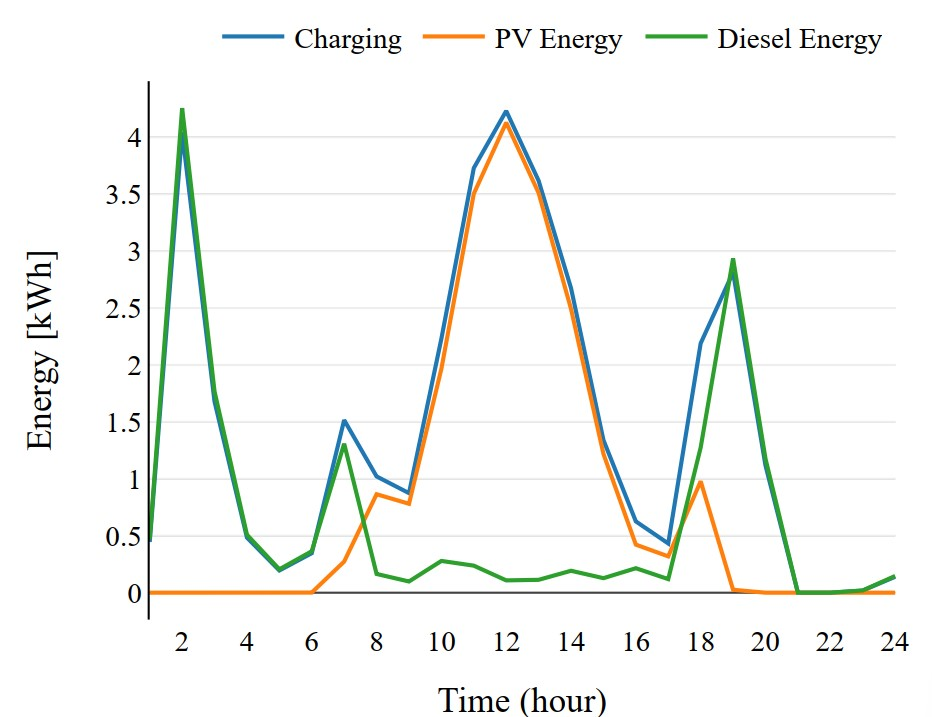
\includegraphics[scale=0.58]{Imágenes/Estado del arte/BESS-PV-DG.jpg}
	\caption{Promedio de energía para cargar el sistema BESS \cite{ropero2022sizing}.}
    \end{center}
\end{figure}

\smallskip

